\section{Individual Generation Process}\label{generationProcess}

If not mentioned differently, each model was trained for 10,000 iterations using a single T4 GPU in Google Colab with the High-Ram setting enabled. It is important to note that this hardware configuration does not match the specifications used in the official implementations of these models. Consequently, the results generated in this study may not be as detailed and precise. Despite these limitations, the primary purpose here is to evaluate the basic capabilities of each model, which is possible even with comparatively modest hardware standards.

To effectively demonstrate the generation process of each method, an example prompt was used: \textbf{``a robot made of plants''}. The choice of this prompt was strategic as concept of a robot is inherently versatile and does not have a rigid definition in terms of appearance or composition. Furthermore, it was assumed that a simple prompt such as \textbf{``a robot''} would lead to bland and colorless models, reflecting the results observed when applying such a prompt to a text-to-image model, specifically Dall-E 3 \citep{dalle3, Dall-E-3}. To mitigate this, the phrase \textbf{``made out of plants''} was added. This not only countered the potential monotony of the models, but also tested the models' ability to represent intricate detail and incorporate color, particularly the various hues associated with plants. The expectation was that this addition would enrich the output of the models and provide a more comprehensive basis for evaluating their detail rendering capabilities.\newline

\textbf{DreamFusion}~--~This method initiates the modeling process with a random scene, which it then incrementally refines throughout the training period. A unique aspect of this method is that each prompt triggers the formation of a new scene, ensuring that even when the same textual input is used repeatedly, it results in the creation of distinct objects. This feature of DreamFusion is showcased through the results visible in Figure~\ref{fig:generationDreamFusion} and Figure~\ref{fig:secondRobotDreamfusion}, both of which are included in the Appendix.
For the purposes of this research, the stable-DreamFusion variant \citep{stable-dreamfusion}, as available in Threestudio, was utilized. This version is distinct from the original DreamFusion implementation, primarily due to the unavailability of Imagen to the public. Details regarding any other modifications made in this version, compared to the original, are outlined in the Appendix~\ref{ch:differences}. 

\begin{figure}[H]
    \centering
    % Subfigure for textual description
    \begin{subfigure}[b]{0.20\textwidth}
        \centering
        \fontsize{9pt}{7pt}\selectfont\text{Iteration 100}\vspace{3cm}
        \fontsize{9pt}{7pt}\selectfont\text{Iteration 5000}\vspace{2.85cm}
        \fontsize{9pt}{7pt}\selectfont\text{Iteration 10000}\vspace{1.95cm}
    \end{subfigure}
    \begin{subfigure}[b]{0.20\textwidth}
        \centering
        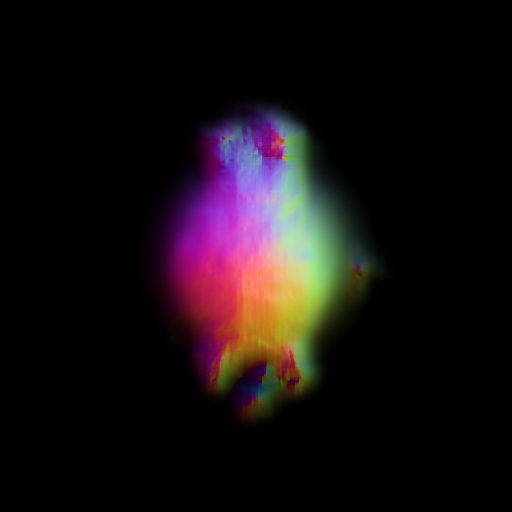
\includegraphics[width=\textwidth]{etc/a robot made out of plants/dreamfusion/dreamfusion_plantrobot_1_part2.png}
        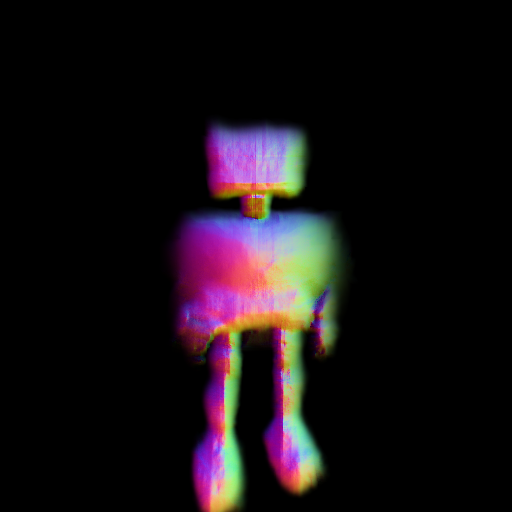
\includegraphics[width=\textwidth]{etc/a robot made out of plants/dreamfusion/dreamfusion_plantrobot_5000_part2.png}
        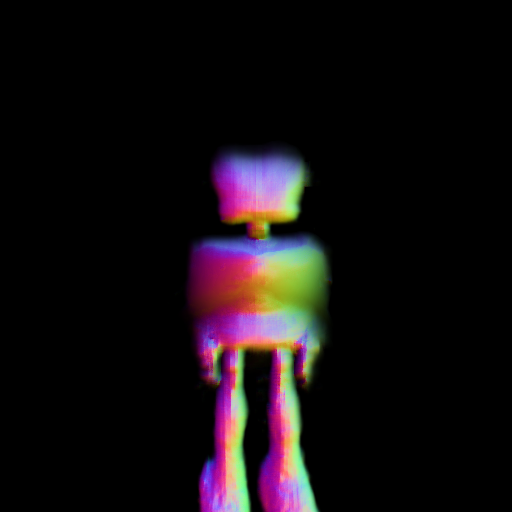
\includegraphics[width=\textwidth]{etc/a robot made out of plants/dreamfusion/dreamfusion_plantrobot_10000_part2.png}
        \caption{}
    \end{subfigure}
    \begin{subfigure}[b]{0.20\textwidth}
        \centering
        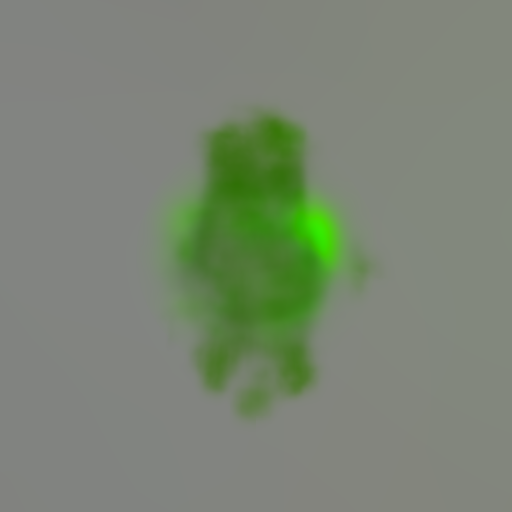
\includegraphics[width=\textwidth]{etc/a robot made out of plants/dreamfusion/dreamfusion_plantrobot_1_part1.png}
        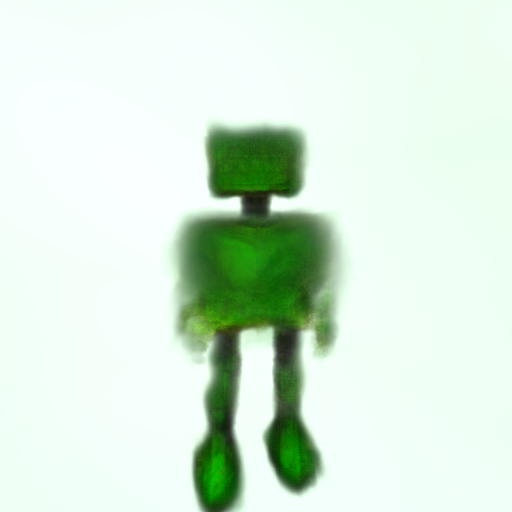
\includegraphics[width=\textwidth]{etc/a robot made out of plants/dreamfusion/dreamfusion_plantrobot_5000_part1.png}
        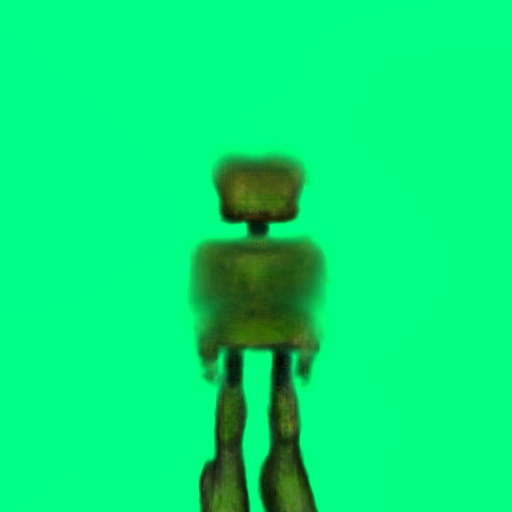
\includegraphics[width=\textwidth]{etc/a robot made out of plants/dreamfusion/dreamfusion_plantrobot_10000_part1.png}
        \caption{}
    \end{subfigure}
    % Subfigure 3
    \hspace{.5cm}
    \begin{subfigure}[b]{0.252\textwidth}
        \centering
        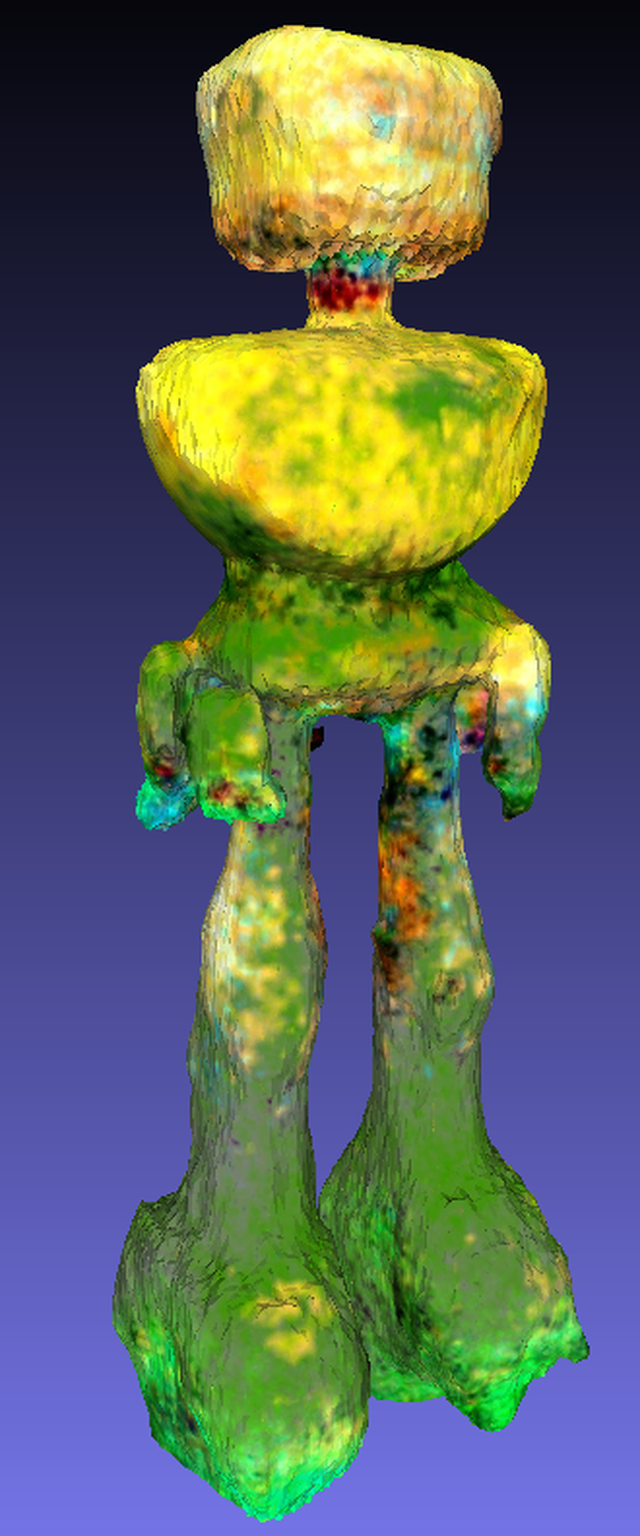
\includegraphics[width=\textwidth]{etc/a robot made out of plants/dreamfusion/dreamfusion_plantrobot_model_resized.png}
        \caption{}
    \end{subfigure}
    \caption{The generation process of DreamFusion using the prompt ``a robot made out of plants''. Section (c) shows a snapshot of the final mesh generated.}~\label{fig:generationDreamFusion}
\end{figure}

As seen in Figure~\ref{fig:generationDreamFusion} parts (a) and (b), the object and its texture are generated simultaneously. The process starts with a small dot that gradually transforms into a more complex shape. At the 100th iteration, the original dot begins to transform into a recognizable shape, and a green hue resembling plant coloration is created. At the 5000th iteration, distinct features such as two legs, a square body and a square head become visible, all retaining the same shade of green. At the last, 10,000th iteration, the model shows a background and small arms sticking out of the robot's body.
Part c of the figure showcases the rendered mesh opened in Meshlab \citep{meshLab}. During the mesh conversion phase, Threestudio made some changes, such as removing duplicates and filling holes. These changes are the reason for the slight differences between the final mesh and the validation images created during training. Interestingly, the final mesh lacks detailed plant-like features, one could only assume that the legs kind of resemble moss, but this remains speculation. The mesh primarily shows basic shapes, including a square head, a torso with small protruding rods that could be arms, and large legs. Remarkably, the upper half of the body in the final mesh takes on a yellowish color that differs from the green of the earlier validation images. The reason for this color change remains unclear.

\textbf{Magic3D}~--~This method employs a coarse-to-fine methodology, aiming to first construct a basic outline of the target object, which is then refined in subsequent stages to more accurately align with the text prompt. The mesh initialization is random, mirroring the approach used in DreamFusion.

\begin{figure}[H]
    \centering
    % Subfigure for textual description
    \begin{subfigure}[b]{0.15\textwidth}
        \centering
        \fontsize{9pt}{7pt}\selectfont\text{Iteration = 200}\vspace{3cm}
        \fontsize{9pt}{7pt}\selectfont\text{It. 5000}\vspace{2.85cm}
        \fontsize{9pt}{7pt}\selectfont\text{It. 10000}\vspace{1.95cm}
    \end{subfigure}
    \begin{subfigure}[b]{0.2\textwidth}
        \centering
        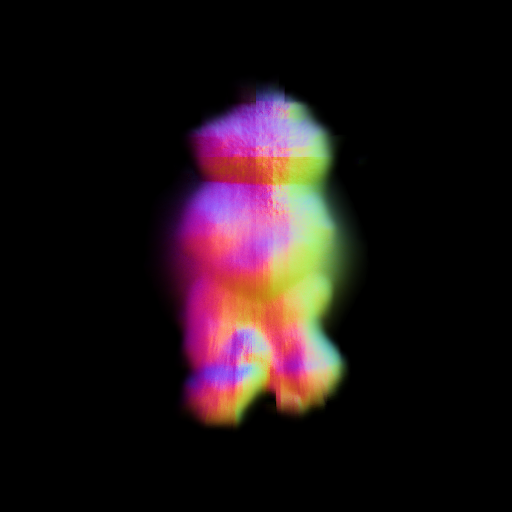
\includegraphics[width=\textwidth]{etc/a robot made out of plants/magic3d/magic3D_coarse_robot_0_part2.png}
        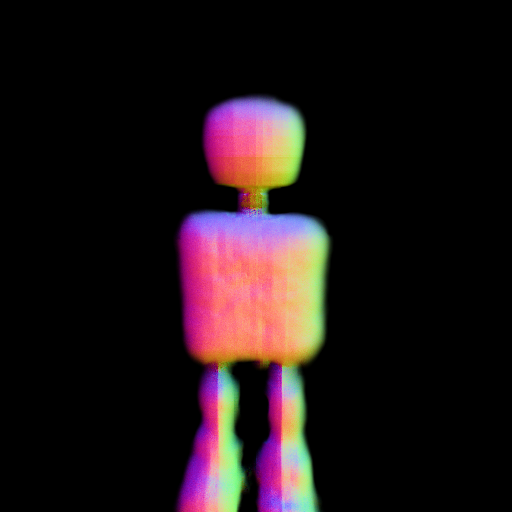
\includegraphics[width=\textwidth]{etc/a robot made out of plants/magic3d/magic3D_coarse_robot_5000_part2.png}
        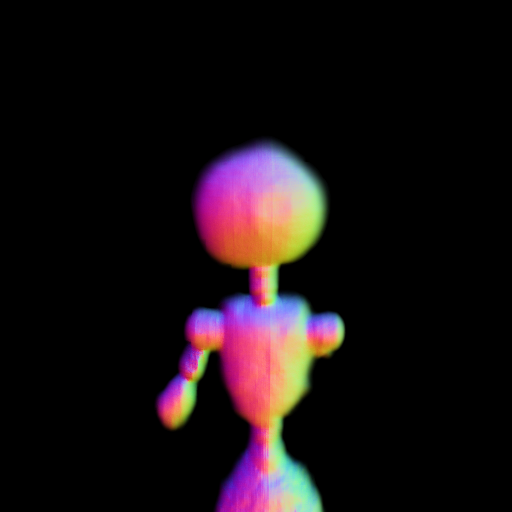
\includegraphics[width=\textwidth]{etc/a robot made out of plants/magic3d/magic3D_coarse_robot_10000_part2.png}
        \caption{}
    \end{subfigure}
    \begin{subfigure}[b]{0.2\textwidth}
        \centering
        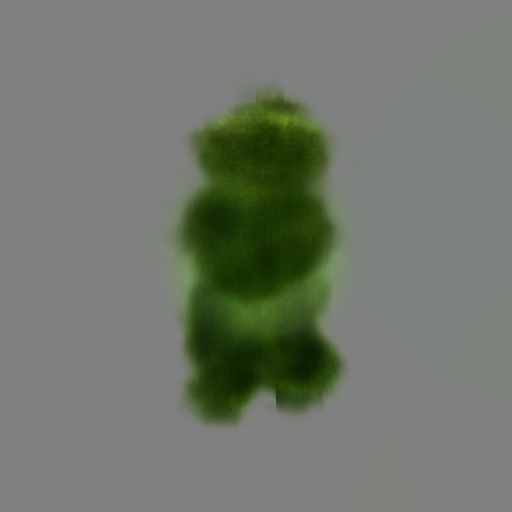
\includegraphics[width=\textwidth]{etc/a robot made out of plants/magic3d/magic3D_coarse_robot_0_part1.png}
        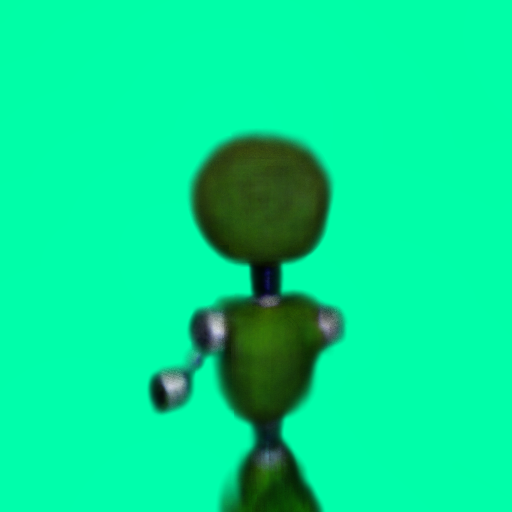
\includegraphics[width=\textwidth]{etc/a robot made out of plants/magic3d/magic3D_coarse_robot_5000_part1.png}
        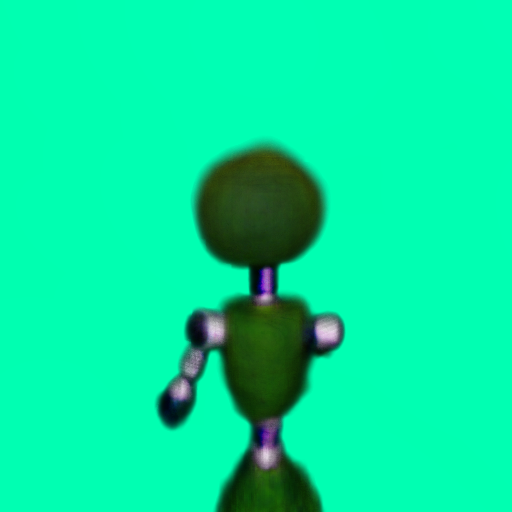
\includegraphics[width=\textwidth]{etc/a robot made out of plants/magic3d/magic3D_coarse_robot_10000_part1.png}
        \caption{}
    \end{subfigure}
    \begin{subfigure}[b]{0.2\textwidth}
        \centering
        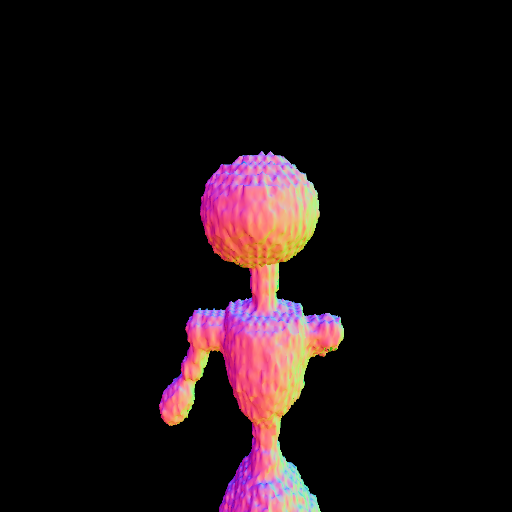
\includegraphics[width=\textwidth]{etc/a robot made out of plants/magic3d/magic3D_refine_robot_0_part2.png}
        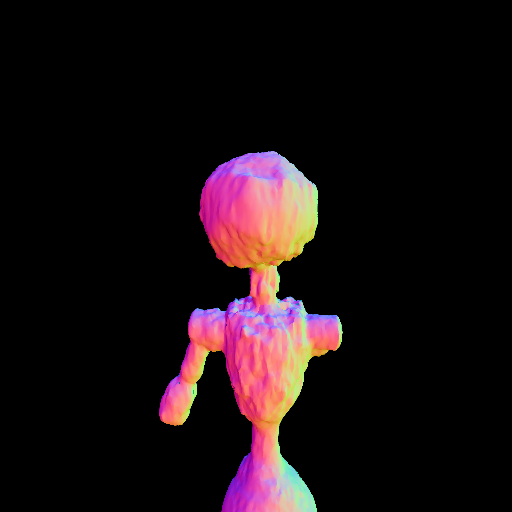
\includegraphics[width=\textwidth]{etc/a robot made out of plants/magic3d/magic3D_refine_robot_5000_part2.png}
        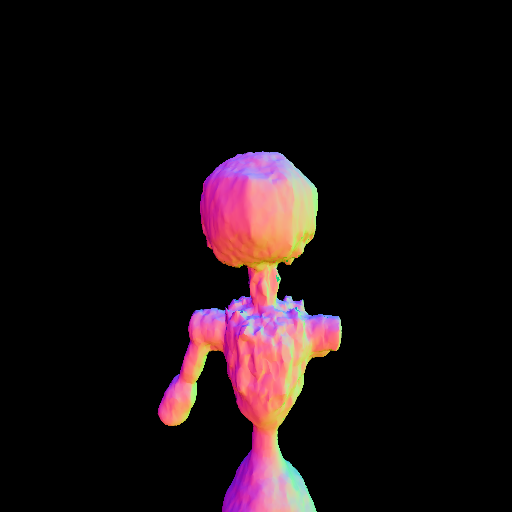
\includegraphics[width=\textwidth]{etc/a robot made out of plants/magic3d/magic3D_refine_robot_10000_part2.png}
        \caption{}
    \end{subfigure}
    \begin{subfigure}[b]{0.2\textwidth}
        \centering
        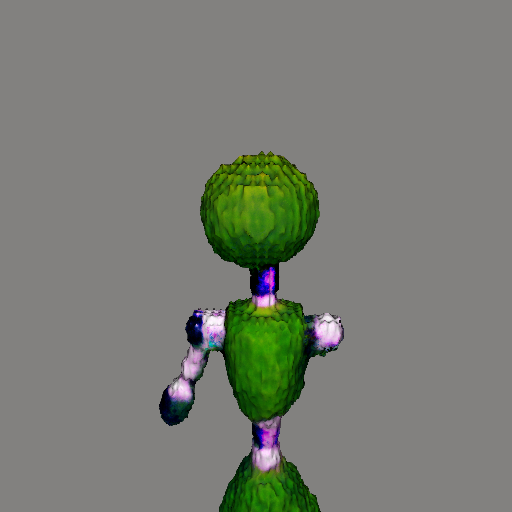
\includegraphics[width=\textwidth]{etc/a robot made out of plants/magic3d/magic3D_refine_robot_0_part1.png}
        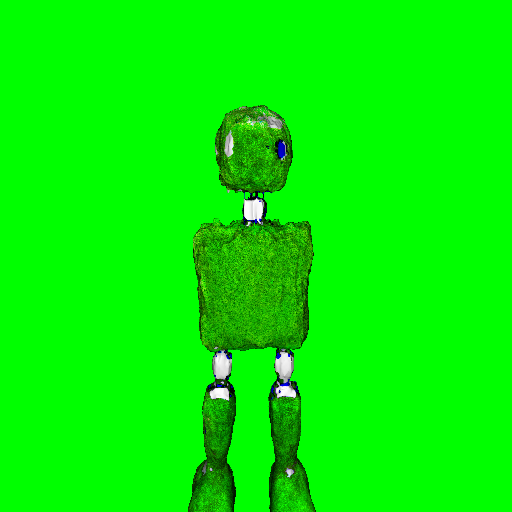
\includegraphics[width=\textwidth]{etc/a robot made out of plants/magic3d/magic3D_refine_robot_5000_part1.png}
        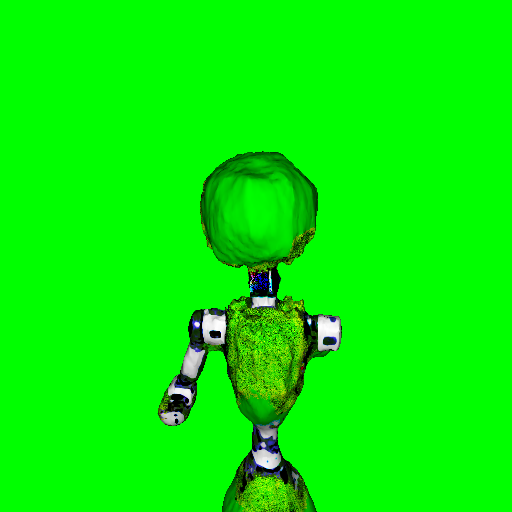
\includegraphics[width=\textwidth]{etc/a robot made out of plants/magic3d/magic3D_refine_robot_10000_part1.png}
        \caption{}
    \end{subfigure}
    \caption{Magic3D generation process from coarse (a, b) to fine (c, d)}~\label{fig:generationMagic3D}
\end{figure} 

The coarse stage can be seen in Figure~\ref{fig:generationMagic3D} parts (a) and (b). From a random start, a rough shape starts emerging by Iteration 200, accompanied by a plant-like green hue, setting the foundation for further refinement. By Iteration 5000, significant transformations have occurred from the initial stage: a distinct circular head, a neck, the upper body of the robot, and one arm have formed. The lower body, however, was omitted during training, forcing subsequent refinements on the upper half. At this point, the arm's color diverges from the green base, taking on a rough, grey-metallic appearance. Progressing to Iteration 10000, the neck and certain parts of the hip also adopt this metallic color. Despite these changes, the overall shape of the model sees only minor adjustments between Iteration 5000 and 10000, such as a thicker left arm and a more pronounced hip, but the right arm remains entirely absent. From the coarse stage alone, the model vaguely indicates a robotic form, with the plant aspect being derived primarily from the green coloring.

In the refinement stage, parts (c) and (d), the process starts from the model generated in the coarse stage. Initially, the mesh appears blocky but retains its original shape, with the neck, shoulder, and hip areas acquiring a purple hue between Iterations 0 and 200. By Iteration 5000, the model is smoother, with minor modifications to the head, losing some of its roundness. However, not much else changes in shape. The texture, though, sees significant refinement; the arms, hip, and neck gain more detail, resembling parts of an actual robot. The chest acquires grass-like detail and coloration. By Iteration 10000, some of these textural details diminish, as evidenced by the stomach area reverting to a plain green. However, the model gains light reflections, particularly noticeable on the shoulders. Despite these changes, the model's shape remains largely unchanged from Iteration 5000 to 10000, and the missing arm issue persists through the refinement stage.

The final mesh, as displayed in Figure~\ref{fig:texturesMagic3D}, is recognizable as a robot, and with close inspection, one might discern its grass-like chest, suggesting a plant-themed robot. For immediate and clear identification, the model would benefit from enhanced detail, particularly a more developed lower body extending beyond the hips. The left side of the figure displays the albedo generated during training.

\begin{figure}[H]
    \centering
      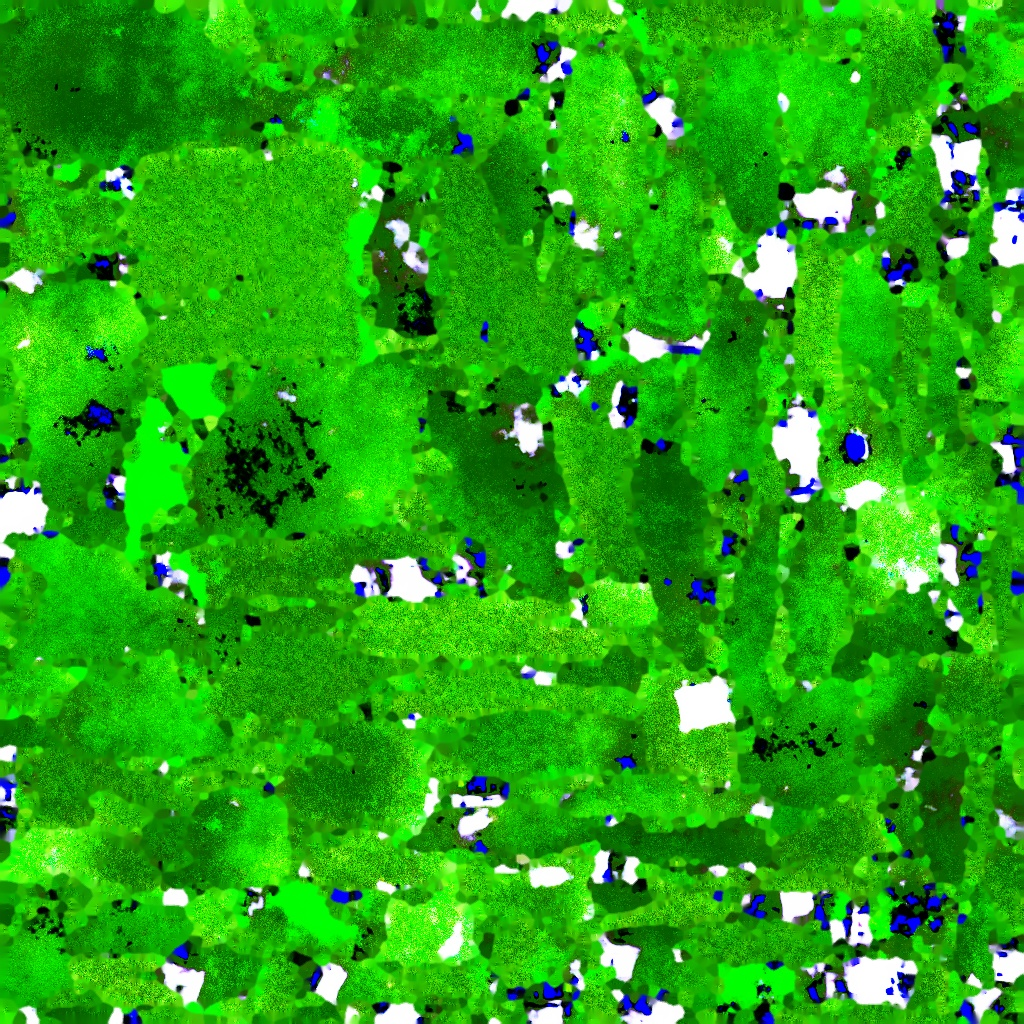
\includegraphics[width=.25\columnwidth]{etc/a robot made out of plants/magic3D/magic3D_refine_robot_texture}
      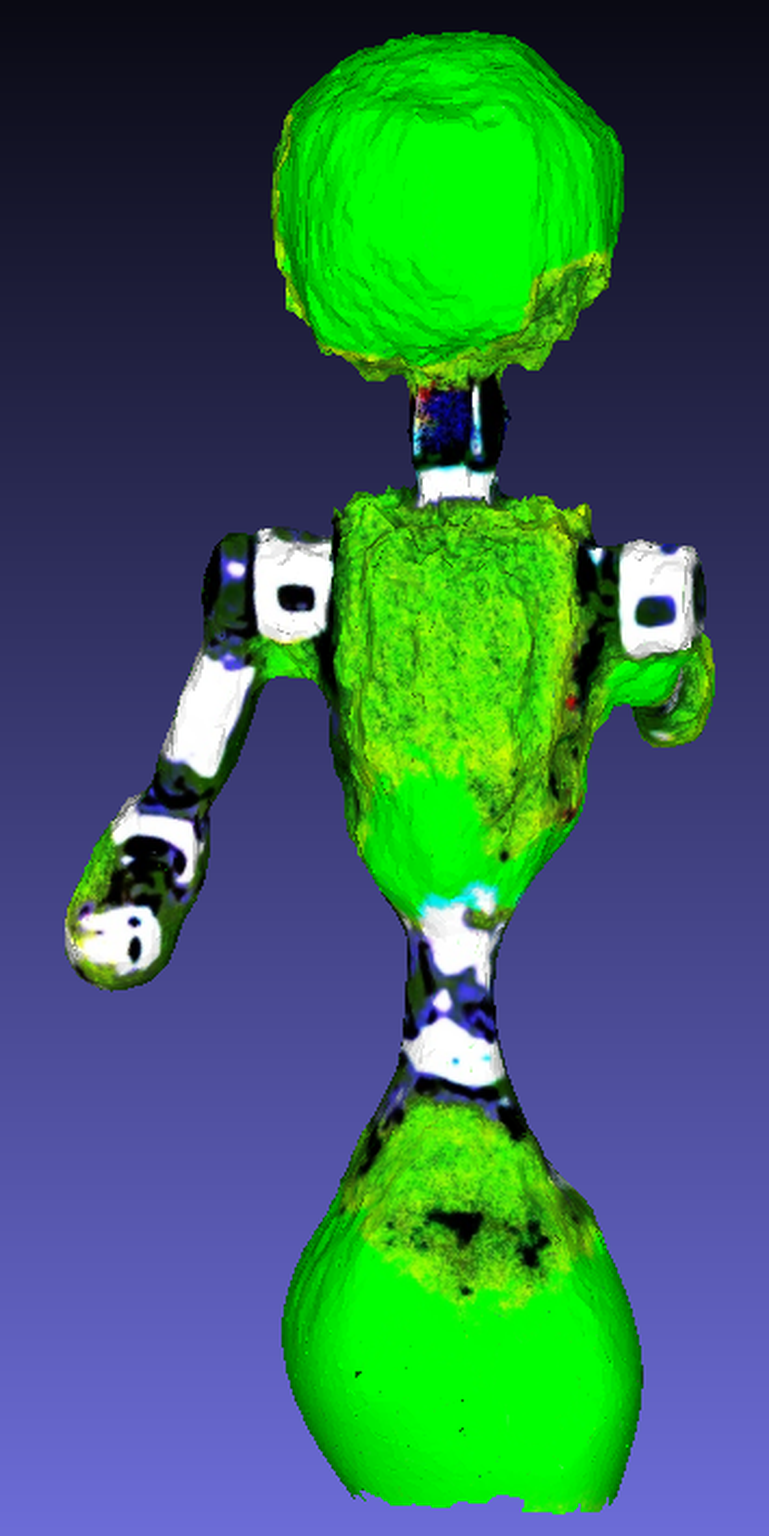
\includegraphics[width=.14\columnwidth]{etc/a robot made out of plants/magic3d/magic3d_plantRobot_model_resized.png}
      \caption{Magic3D also generates an albedo during training. The right side shows the extracted mesh.}~\label{fig:texturesMagic3D}
\end{figure}

\indent\textbf{Fantasia3D}~--~There are several ways to initiate the generation of 3D models in Fantasia3D. The most straightforward method, used in this section, is to begin with just the prompt, wherein Fantasia3D defaults to using a sphere as the initial mesh, shaping the training process from this starting point. Alternatively, one can customize the sphere's initial values  \([0.5, 0.5, 0.5]\) to better represent the desired object by adjusting the parameters to correspond to \([depth, width, height]\). The final approach involves initializing the mesh with a custom~.obj file, providing a rough outline of the intended shape. An example of the latter approach can be seen in Figure~\ref{fig:generationFantasia2} in the appendix, where the generation process was started with a rough human figure.

\begin{figure}[H]
    \centering
    % Subfigure for textual description
    \begin{subfigure}[b]{0.20\textwidth}
        \centering
        \fontsize{9pt}{7pt}\selectfont\text{Iteration 0}\vspace{3cm}
        \fontsize{9pt}{7pt}\selectfont\text{Iteration 5000}\vspace{2.85cm}
        \fontsize{9pt}{7pt}\selectfont\text{Iteration 10000}\vspace{1.95cm}
    \end{subfigure}
    \begin{subfigure}[b]{0.20\textwidth}
        \centering
        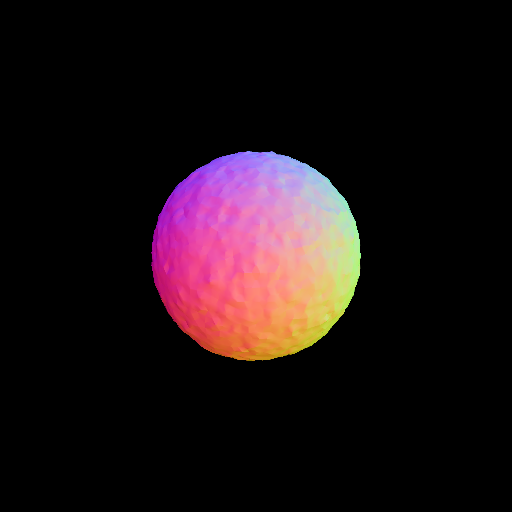
\includegraphics[width=\textwidth]{etc/a robot made out of plants/fantasia3d/fantasia_coarse_robot_0_part2.png}
        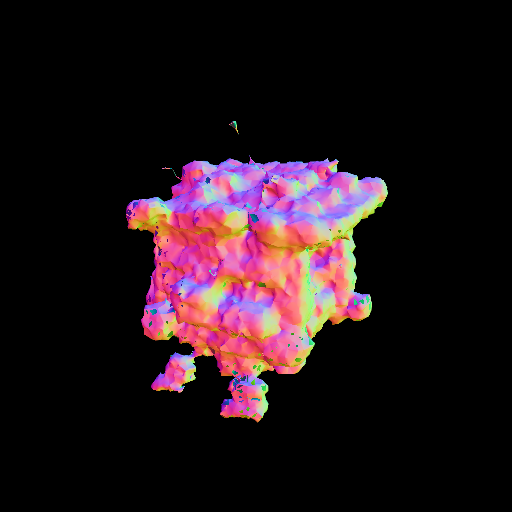
\includegraphics[width=\textwidth]{etc/a robot made out of plants/fantasia3d/fantasia_coarse_robot_5000_part2.png}
        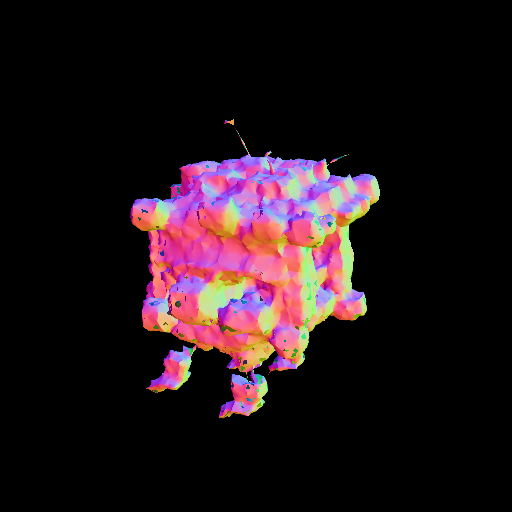
\includegraphics[width=\textwidth]{etc/a robot made out of plants/fantasia3d/fantasia_coarse_robot_10000_part2.png}
        \caption{}
    \end{subfigure}
    \begin{subfigure}[b]{0.20\textwidth}
        \centering
        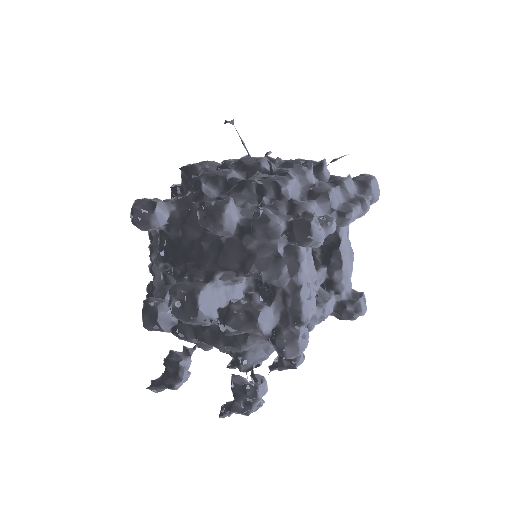
\includegraphics[width=\textwidth]{etc/a robot made out of plants/fantasia3d/fantasia_refine_robot_0_part1.png}
        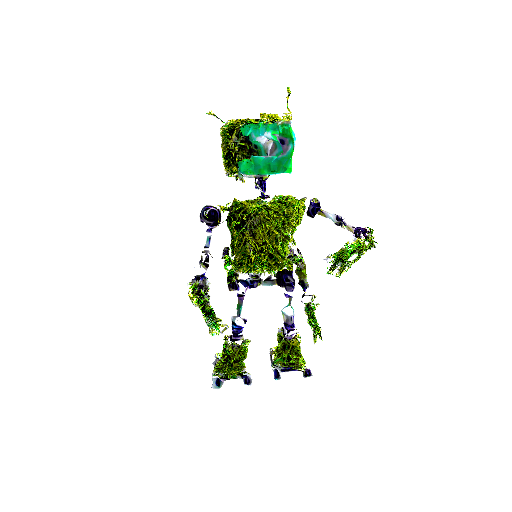
\includegraphics[width=\textwidth]{etc/a robot made out of plants/fantasia3d/fantasia_refine_robot_5000_part1.png}
        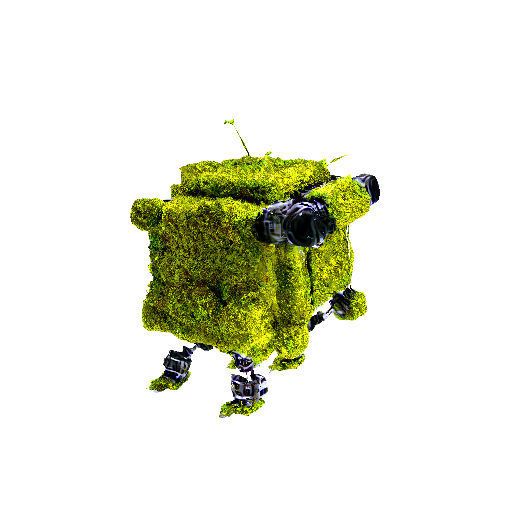
\includegraphics[width=\textwidth]{etc/a robot made out of plants/fantasia3d/fantasia_refine_robot_10000_part1.png}
        \caption{}
    \end{subfigure}
    % Subfigure 3
    \begin{subfigure}[b]{0.37\textwidth}
        \centering
        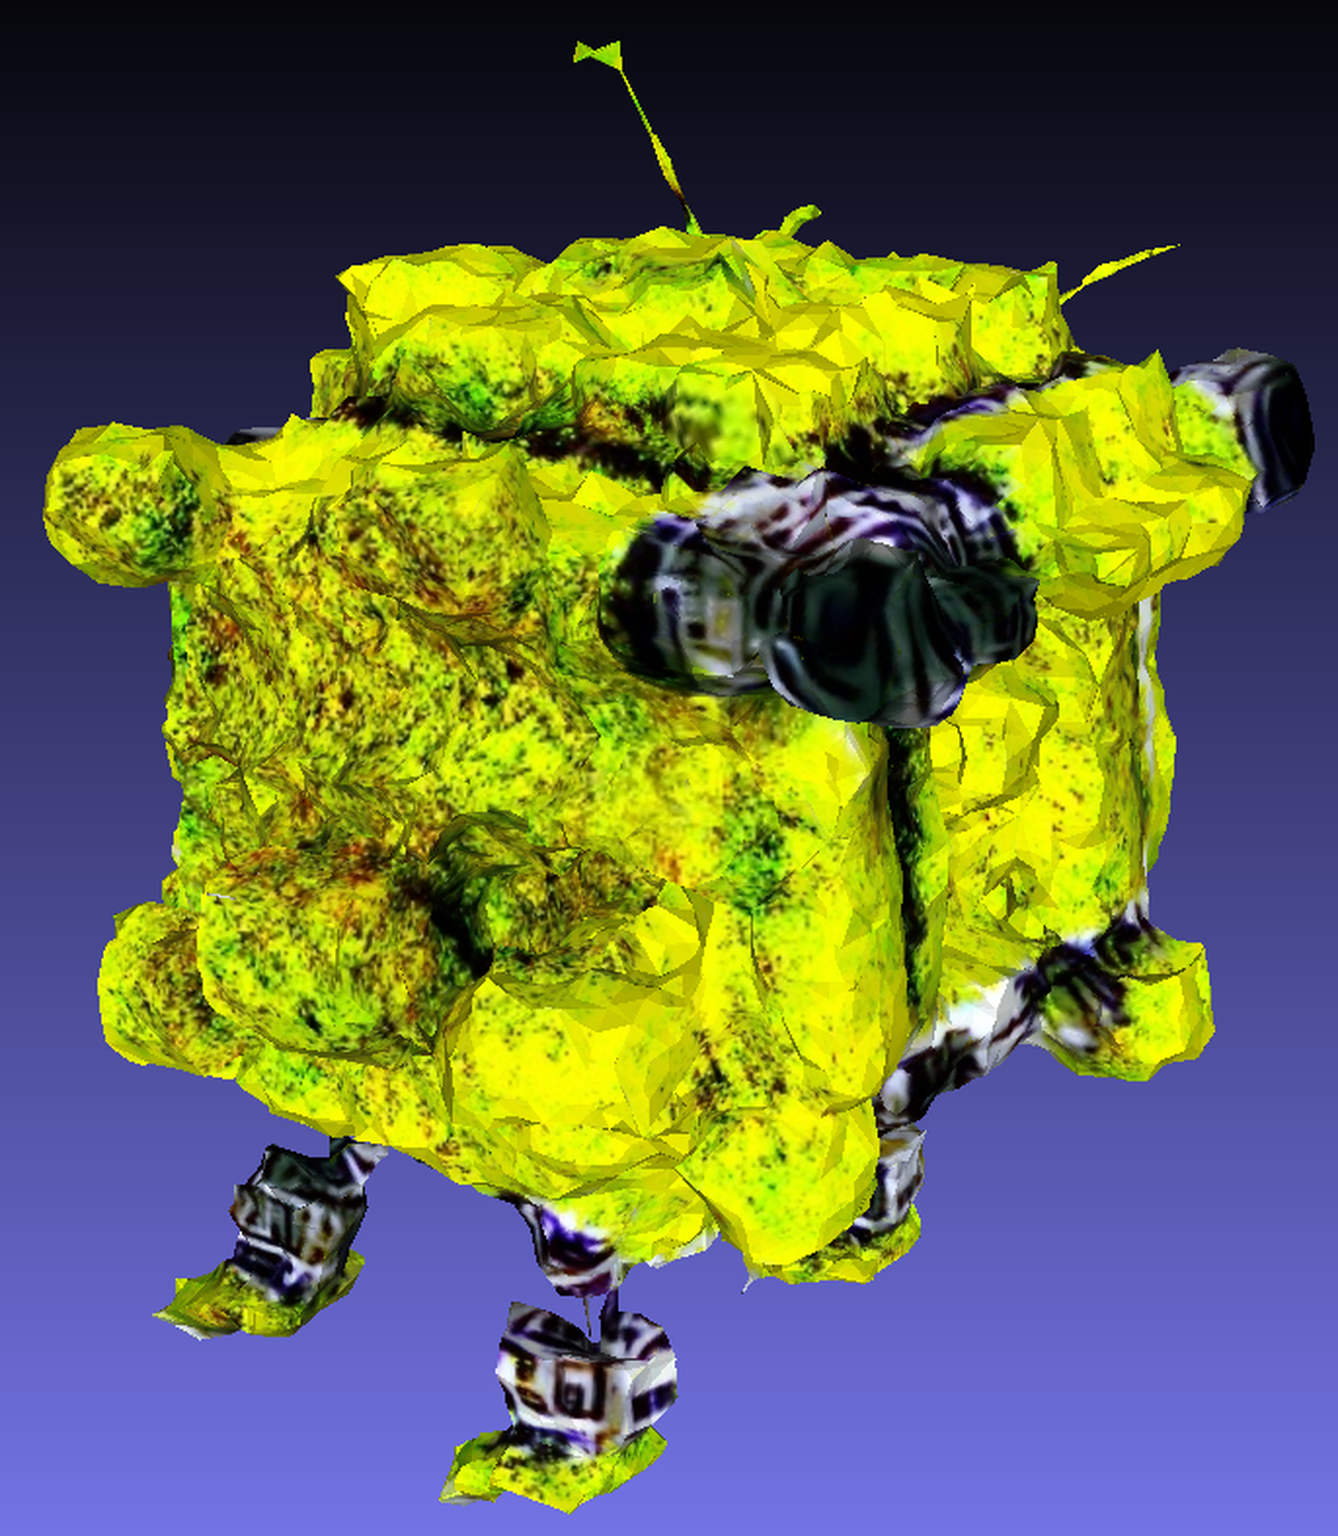
\includegraphics[width=\textwidth]{etc/a robot made out of plants/fantasia3d/fantasia_plantrobot_model_resized.png}
        \caption{}
    \end{subfigure}
    \caption{Fantasia3D's results: Part (a) illustrates the geometric evolution of the model, while part (b) showcases the development of the model's appearance. Part (c) presents the final rendered model as viewed in Meshlab.}~\label{fig:generationFantasia}
\end{figure}

Part (a) of Figure~\ref{fig:generationFantasia} illustrates the geometry stage of the method. Since only the prompt was used for initialization, Fantasia3D automatically selected a sphere as the base, influencing the overall quadratic shape of the final model. The figure reveals that the majority of the transformations occur between iterations 0 and 5000, where the sphere evolves, gaining corners and forming smaller blocks at the bottom, potentially interpreted as the robot's feet. However, at this geometry stage, it's challenging to discern the robot, especially as one made of plants. The changes from iteration 5000 to 10000 are more subtle, with slight smoothing in certain areas, such as the block on the top left side of the robot or parts of the left foot, but these alterations are not significantly transformative.

Part (b) of the figure displays the appearance stage, where the model is textured. Starting with a textureless base derived from the previous stage, the model gains color and texture as iterations progress. By iteration 5000, the texture, surprisingly resembling grass, enhances the model's detail and color, diminishing the prominence of the earlier clunky geometry. From iteration 5000 to 10000, this texture is further refined, introducing more detailed color variations and shadows, simulating light effects. Additionally, certain areas of the model exhibit metallic grey tones, particularly noticeable at the top right side and between the main body and the feet. 

However, some of these textural details are lost in the final mesh extraction, as seen in part (c). The model takes on a more yellowish hue, and the previously distinct lighting and shadows are reduced. Similar to the geometry stage, the final model does not clearly represent a robot made of plants; it more closely resembles a box with feet, akin to robots designed for food delivery. Throughout the training, Fantasia3D also generates various textures, including diffuse, roughness, metallic, and normals, as depicted in Figure~\ref{fig:texturesFantasia}.

\begin{figure}[H]
    \centering
      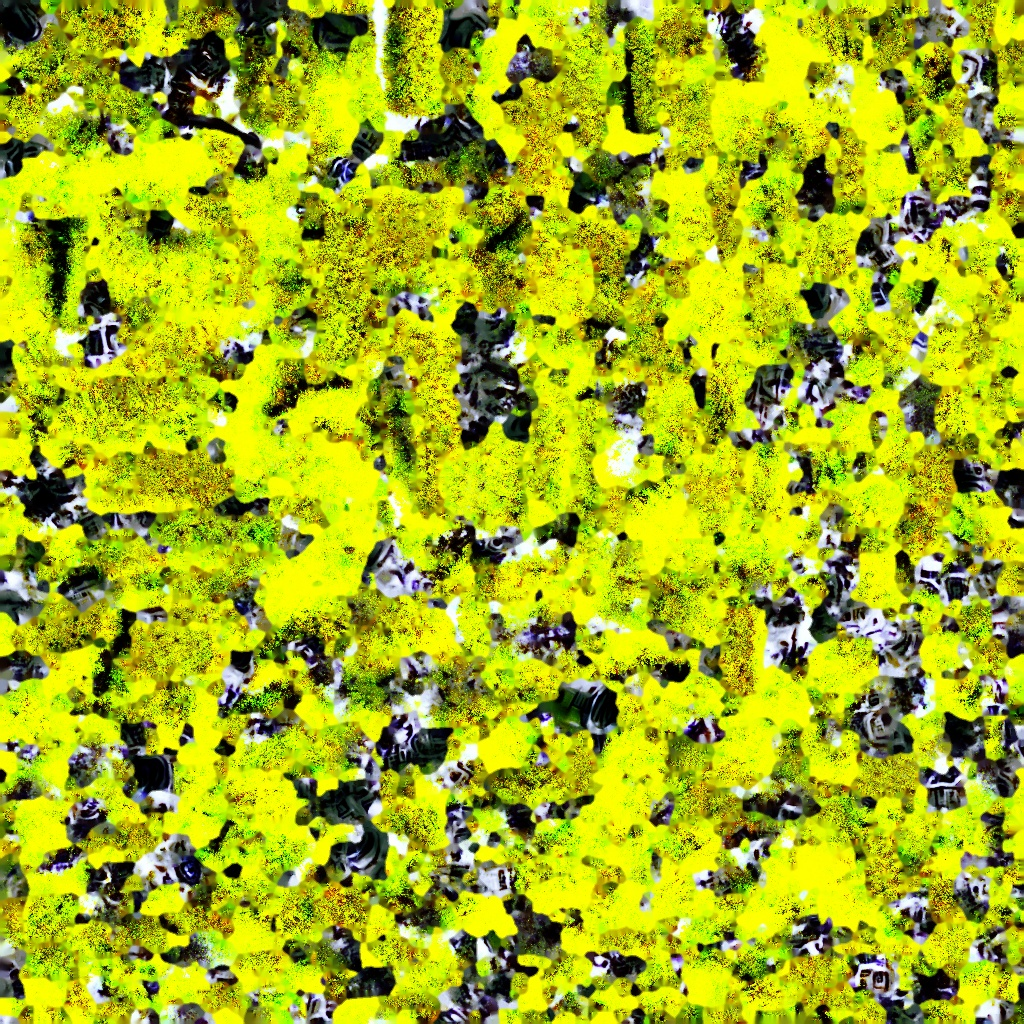
\includegraphics[width=.15\columnwidth]{etc/a robot made out of plants/fantasia3d/fantasia_refine_robot_kd}
      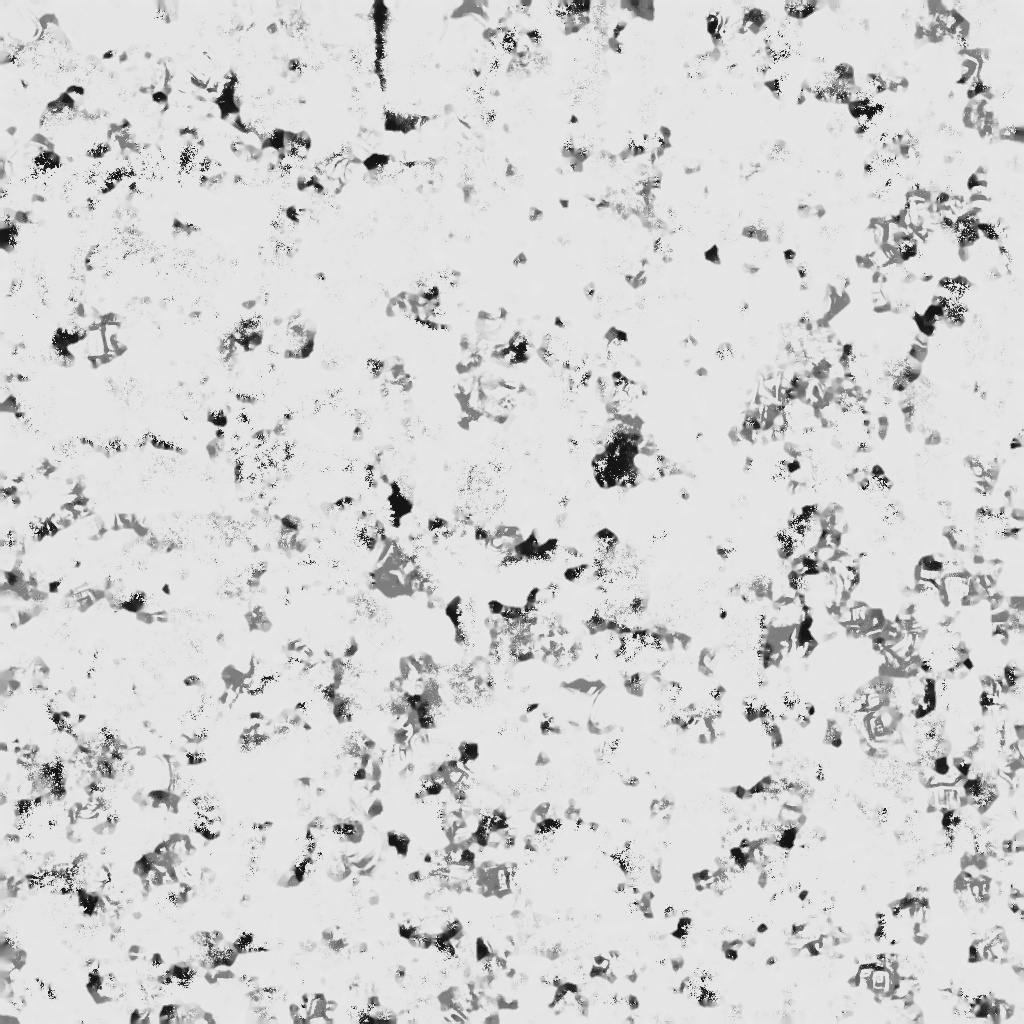
\includegraphics[width=.15\columnwidth]{etc/a robot made out of plants/fantasia3d/fantasia_refine_robot_roughness}
      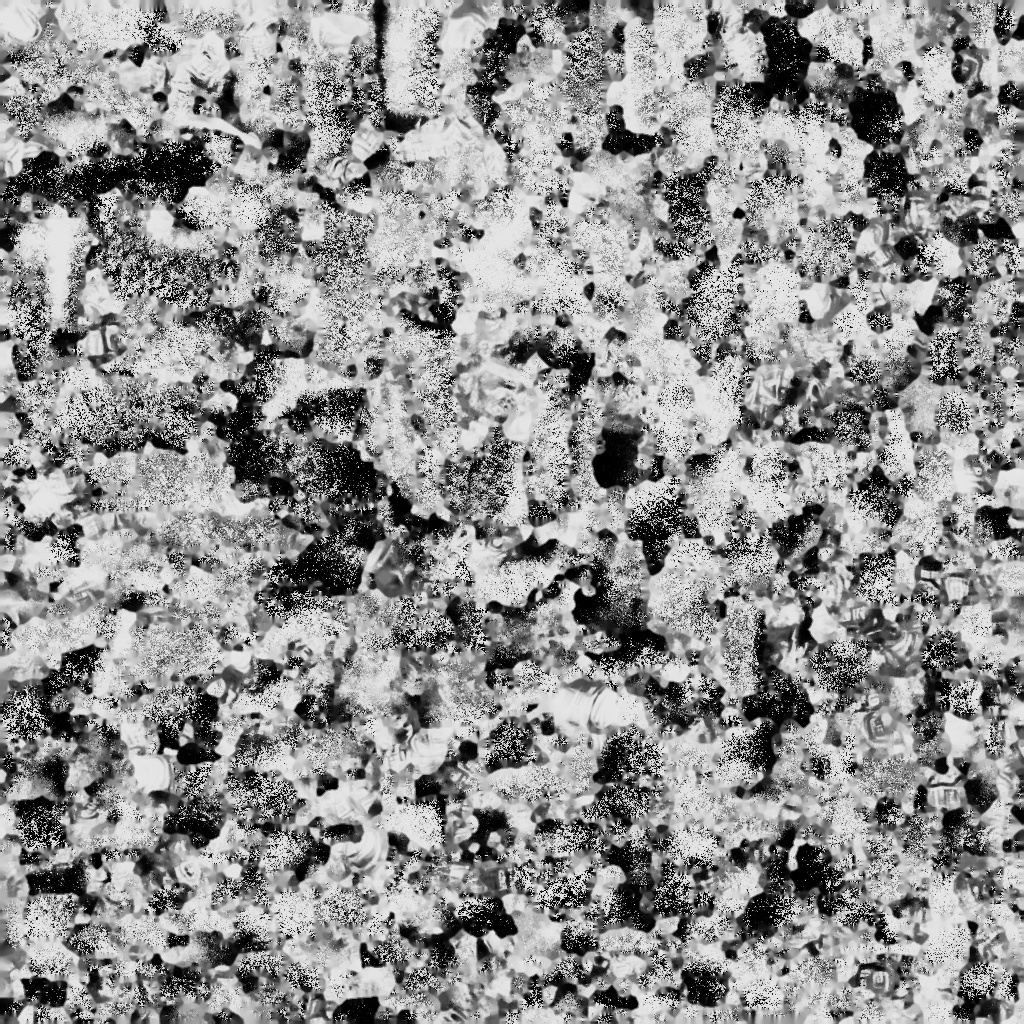
\includegraphics[width=.15\columnwidth]{etc/a robot made out of plants/fantasia3d/fantasia_refine_robot_metallic}
      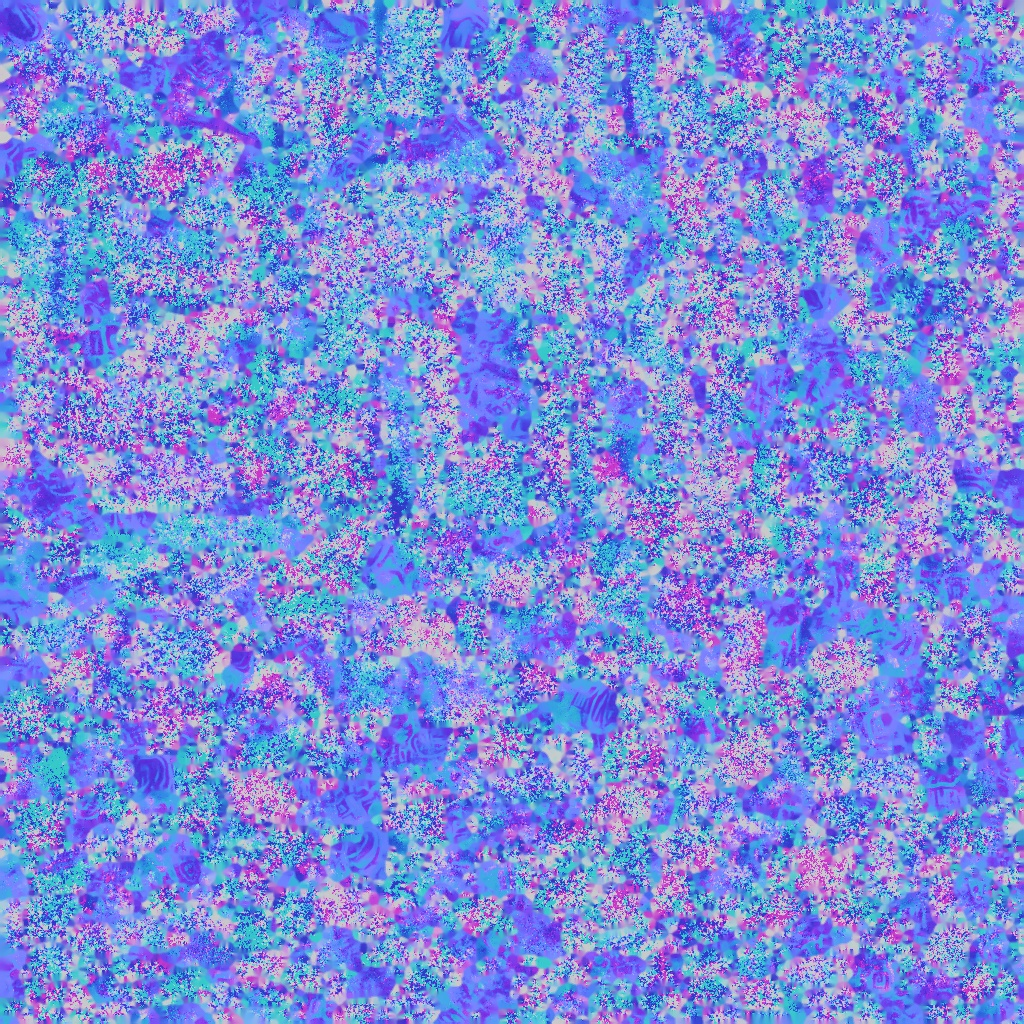
\includegraphics[width=.15\columnwidth]{etc/a robot made out of plants/fantasia3d/fantasia_refine_robot_normal}
      \caption{Generated textures from Fantasia3D\@; from left to right:  diffuse, roughness, metallic, and normal.}~\label{fig:texturesFantasia}
  \end{figure}
\textbf{Magic123}~--~Magic123 employs a unique approach that integrates both 2D and 3D priors for generating 3D objects. The method initiates by processing an input image, creating multiple perspectives of the intended object. The initial phase involves constructing a low-quality, coarse model complete with texture, forming a basic representation of the object. Subsequently, this model undergoes a refinement stage, where additional details are added to both the object and its texture.

\begin{figure}[H]
    \centering
    % Subfigure for textual description
    \begin{subfigure}[b]{0.25\textwidth}
        \centering
        \fontsize{9pt}{7pt}\selectfont\text{Iteration = 100}\vspace{.1cm}
        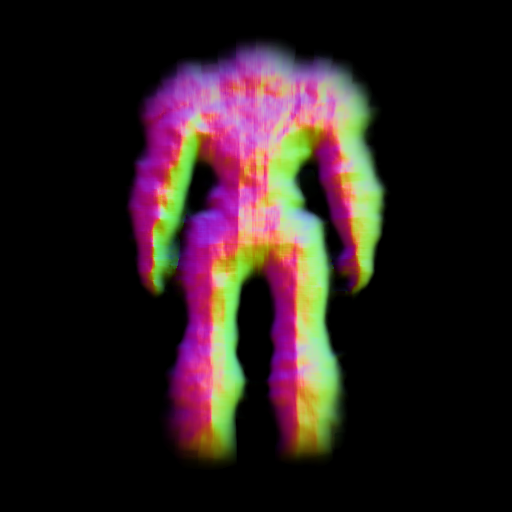
\includegraphics[width=\textwidth]{etc/a robot made out of plants/magic123/magic123_coarse_robot_front_0_part2.png}
        
\includegraphics[width=\textwidth]{etc/a robot made out of plants/magic123/magic123_coarse_robot_front_0_part1.png}
        \caption{}
    \end{subfigure}
    \begin{subfigure}[b]{0.25\textwidth}
        \centering
        \fontsize{9pt}{7pt}\selectfont\text{Iteration = 5000}\vspace{.1cm}
        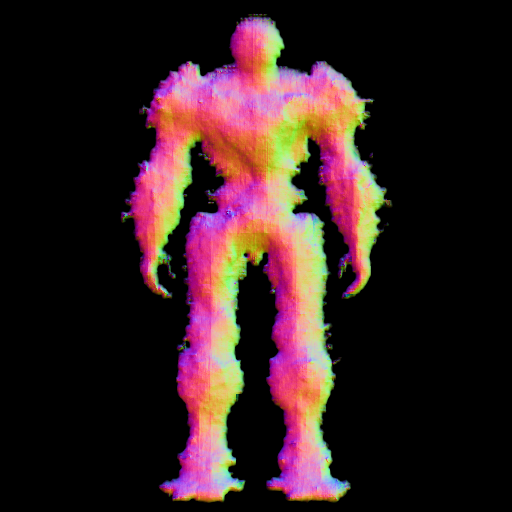
\includegraphics[width=\textwidth]{etc/a robot made out of plants/magic123/magic123_coarse_robot_front_5000_part2.png}
        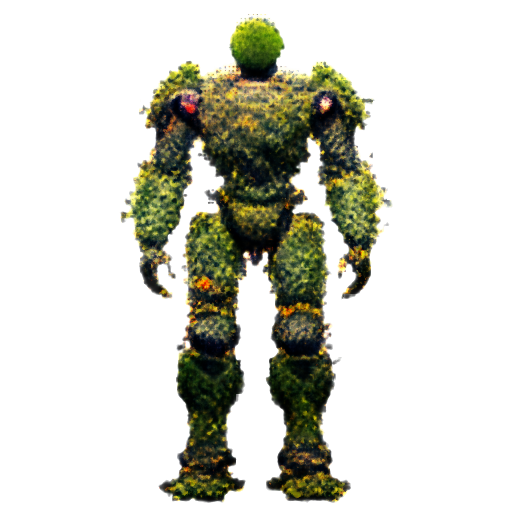
\includegraphics[width=\textwidth]{etc/a robot made out of plants/magic123/magic123_coarse_robot_front_5000_part1.png}
        \caption{}
    \end{subfigure}
    \begin{subfigure}[b]{0.25\textwidth}
        \centering
        \fontsize{9pt}{7pt}\selectfont\text{Iteration = 10000}\vspace{.1cm}
        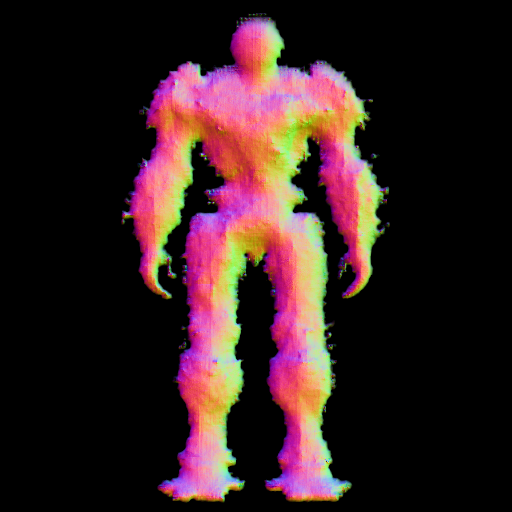
\includegraphics[width=\textwidth]{etc/a robot made out of plants/magic123/magic123_coarse_robot_front_10000_part2.png}
        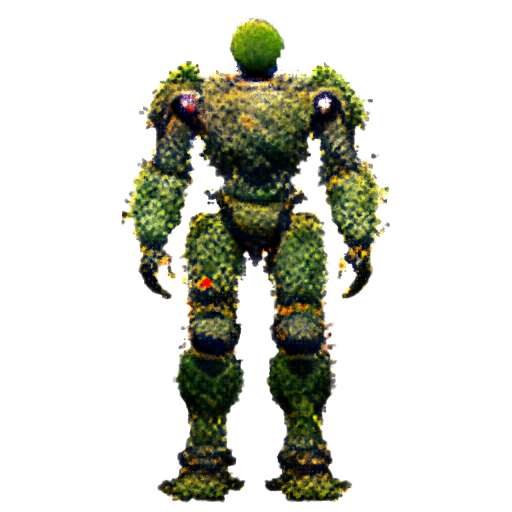
\includegraphics[width=\textwidth]{etc/a robot made out of plants/magic123/magic123_coarse_robot_front_10000_part1.png}
        \caption{}
    \end{subfigure}
    \caption{Front view of the coarse stage of Magic123}~\label{fig:generationFrontCoarseMagic123}
\end{figure}

The front view of the coarse generation process is depicted in Figure~\ref{fig:generationFrontCoarseMagic123}. Even at an early stage like Iteration 100, the method efficiently produces an outline that resonates well with the input image, including the incorporation of a green hue to represent the plant aspects. Progressing to Iteration 5000, the model becomes more detailed, with sharper edges and a more defined robotic shape. Elements suggestive of overgrowth, such as leaves and vines, begin to emerge, and the texture convincingly integrates plant-like features, covering the model with grass and vine patterns. By Iteration 10000 in this stage, the model's shape does not evolve significantly, but some color variation in the plant textures and distinct features like a white spot on the right shoulder and a bright red dot above the left knee emerge, hinting at metallic robot parts and a blooming flower, respectively.

During the refinement stage, showcased in Figure~\ref{fig:generationFrontRefineMagic123}, the model initially loses some of its detailed and mossy character from the coarse stage. Floating parts disconnected from the main body become noticeable, particularly on the right arm and the left leg. Compared to the 10000th iteration of the coarse stage, the texture seems less detailed initially. However, by Iteration 5000, the texture regains and even surpasses its former level of detail, presenting a more realistic plant-like structure. The model appears covered in grass, moss, and vines, with enhanced features like a more pronounced blooming flower and more defined hands, knees, shoulders, and feet. Further into Iteration 10000, the model becomes smoother, particularly around the thighs and chest, though the floating parts persist. The texture at this stage is remarkably detailed, offering a realistic plant appearance with effective light and shadow interplay, particularly around the stomach area.

\begin{figure}[H]
    \centering
    % Subfigure for textual description
    \begin{subfigure}[b]{0.25\textwidth}
        \centering
        \fontsize{9pt}{7pt}\selectfont\text{Iteration = 100}\vspace{.1cm}
        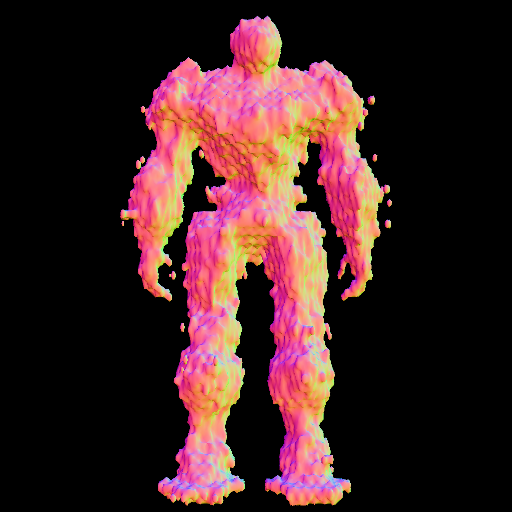
\includegraphics[width=\textwidth]{etc/a robot made out of plants/magic123/magic123_refine_robot_front_0_part2.png}
        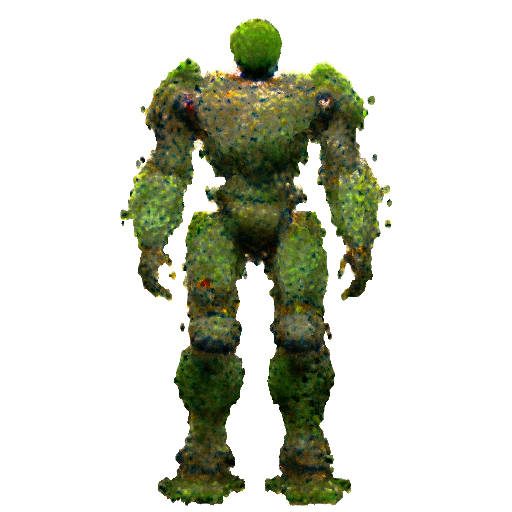
\includegraphics[width=\textwidth]{etc/a robot made out of plants/magic123/magic123_refine_robot_front_0_part1.png}
        \caption{}
    \end{subfigure}
    \begin{subfigure}[b]{0.25\textwidth}
        \centering
        \fontsize{9pt}{7pt}\selectfont\text{Iteration = 5000}\vspace{.1cm}
        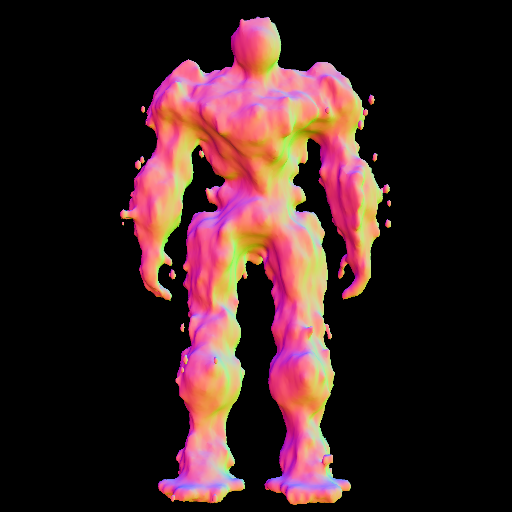
\includegraphics[width=\textwidth]{etc/a robot made out of plants/magic123/magic123_refine_robot_front_5000_part2.png}
        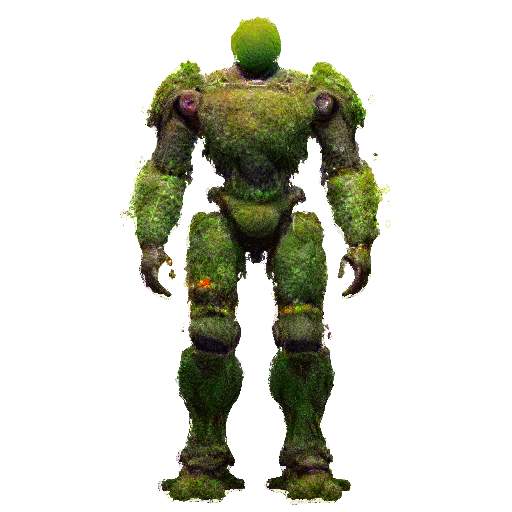
\includegraphics[width=\textwidth]{etc/a robot made out of plants/magic123/magic123_refine_robot_front_5000_part1.png}
        \caption{}
    \end{subfigure}
    \begin{subfigure}[b]{0.25\textwidth}
        \centering
        \fontsize{9pt}{7pt}\selectfont\text{Iteration = 10000}\vspace{.1cm}
        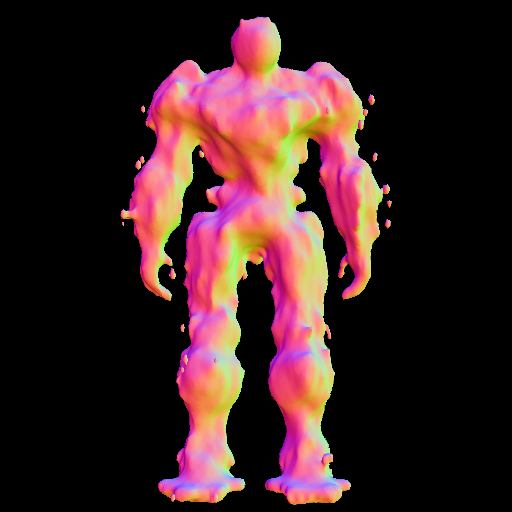
\includegraphics[width=\textwidth]{etc/a robot made out of plants/magic123/magic123_refine_robot_front_10000_part2.png}
        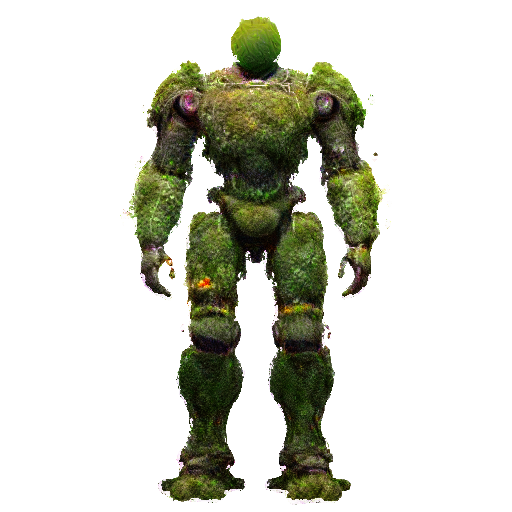
\includegraphics[width=\textwidth]{etc/a robot made out of plants/magic123/magic123_refine_robot_front_10000_part1.png}
        \caption{}
    \end{subfigure}
    \caption{Front view of the refine stage of Magic123}~\label{fig:generationFrontRefineMagic123}
\end{figure}

As Magic123 generates multiple views during training, additional perspectives of the object for each iteration can be seen in Figures~\ref{fig:generationCoarseMagic123} and~\ref{fig:generationRefineMagic123} in the appendix, which include the right, back, and left views. In there one can see the difficulties magic123 had in the beginning while determining the side views of the model. These problems however quickly dissapeared until Iteration 5000. 

The final mesh, as illustrated in part (a) of Figure~\ref{fig:inputAndModel}, exhibits reasonable quality. Some white spots, particularly around the floating parts, suggest that these areas may remain textureless due to rendering issues. In comparison, the final model does a commendable job in mirroring the overall shape of the input image, as seen in part (b) of the same figure. Despite this, it becomes evident that Magic123 struggles to replicate the complex details of the plants. This shortcoming highlights the limitations of the method when it comes to fully capturing and translating the details in the input image into the 3D model. However, longer training iterations and higher computing power could mitigate this.

\begin{figure}[H]
    \centering
    \begin{subfigure}[b]{0.23\textwidth}
        \centering
        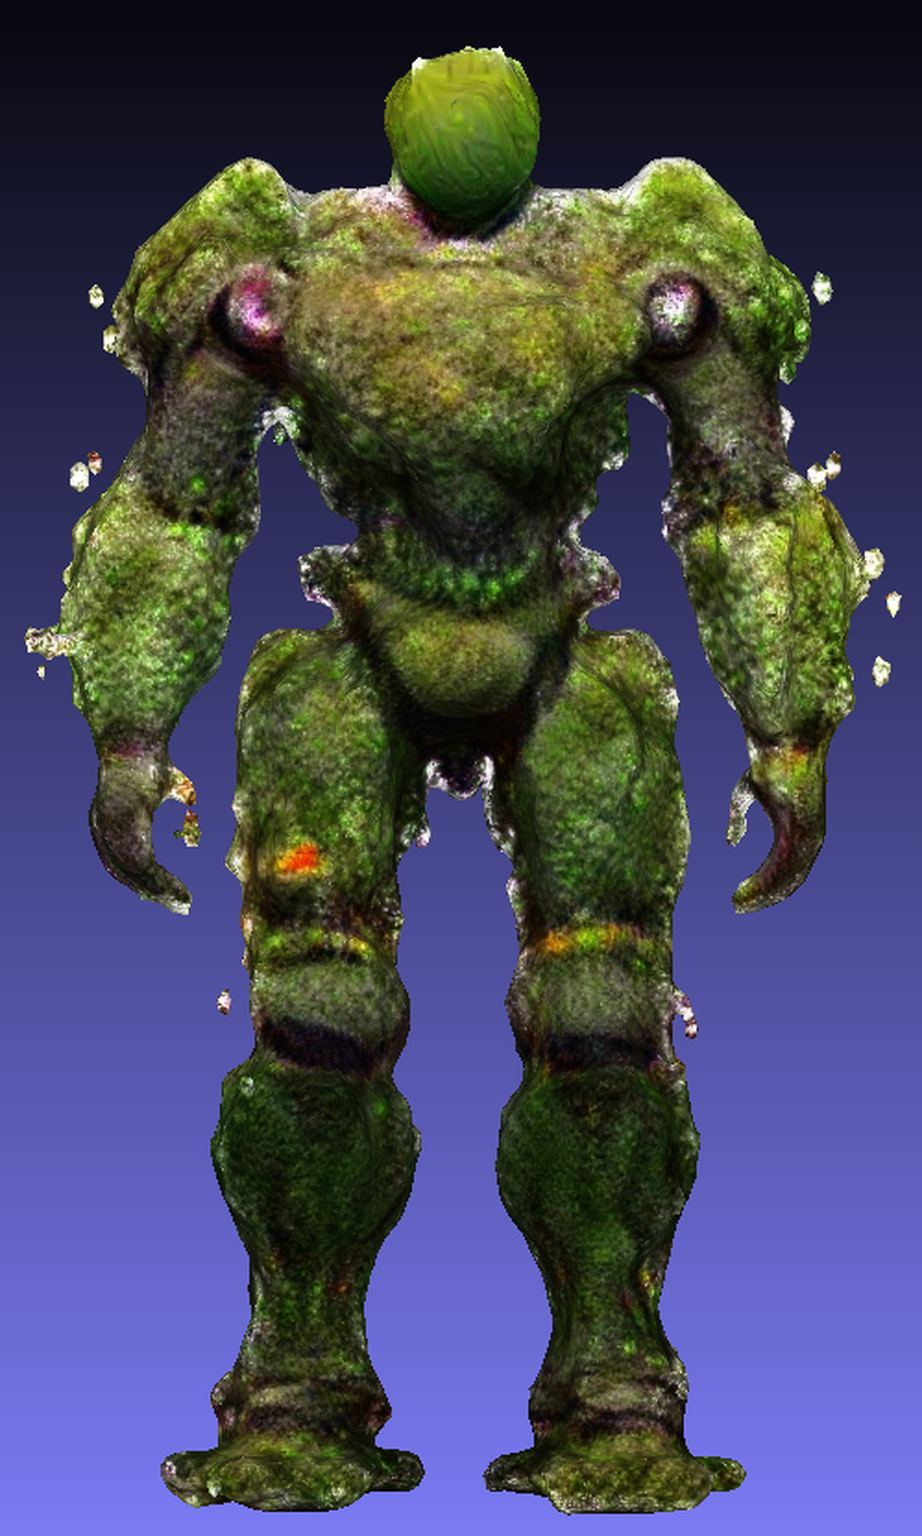
\includegraphics[width=\textwidth]{etc/a robot made out of plants/magic123/magic123_plantRobot_model_resized.png}
        \caption{Magic123}
    \end{subfigure}
    \begin{subfigure}[b]{0.38\textwidth}
        \centering
        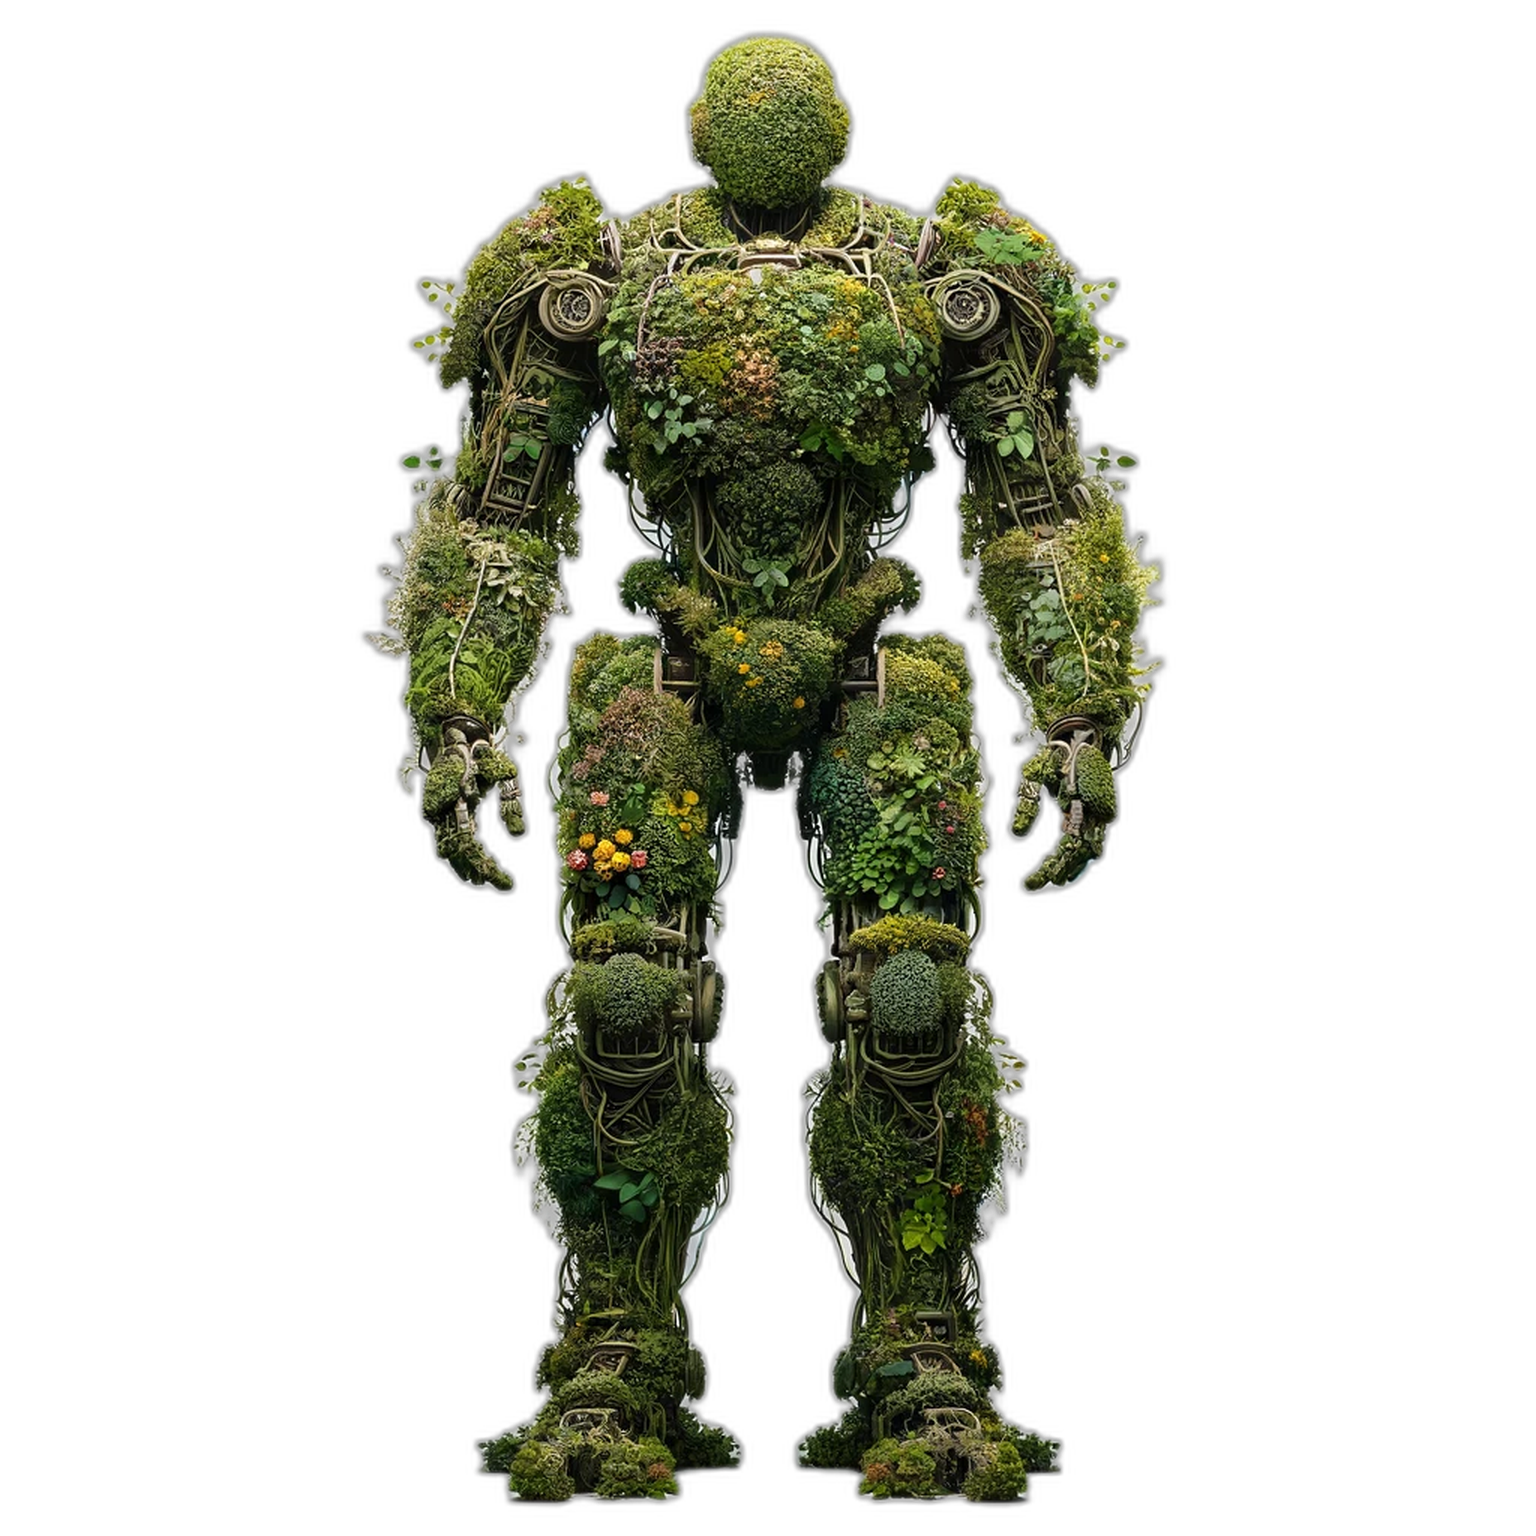
\includegraphics[width=\textwidth]{etc/a robot made out of plants/magic123/robot made out of plants_noBG_resized.png}
        \caption{Input Image}
    \end{subfigure}
    \begin{subfigure}[b]{0.21\textwidth}
        \centering
        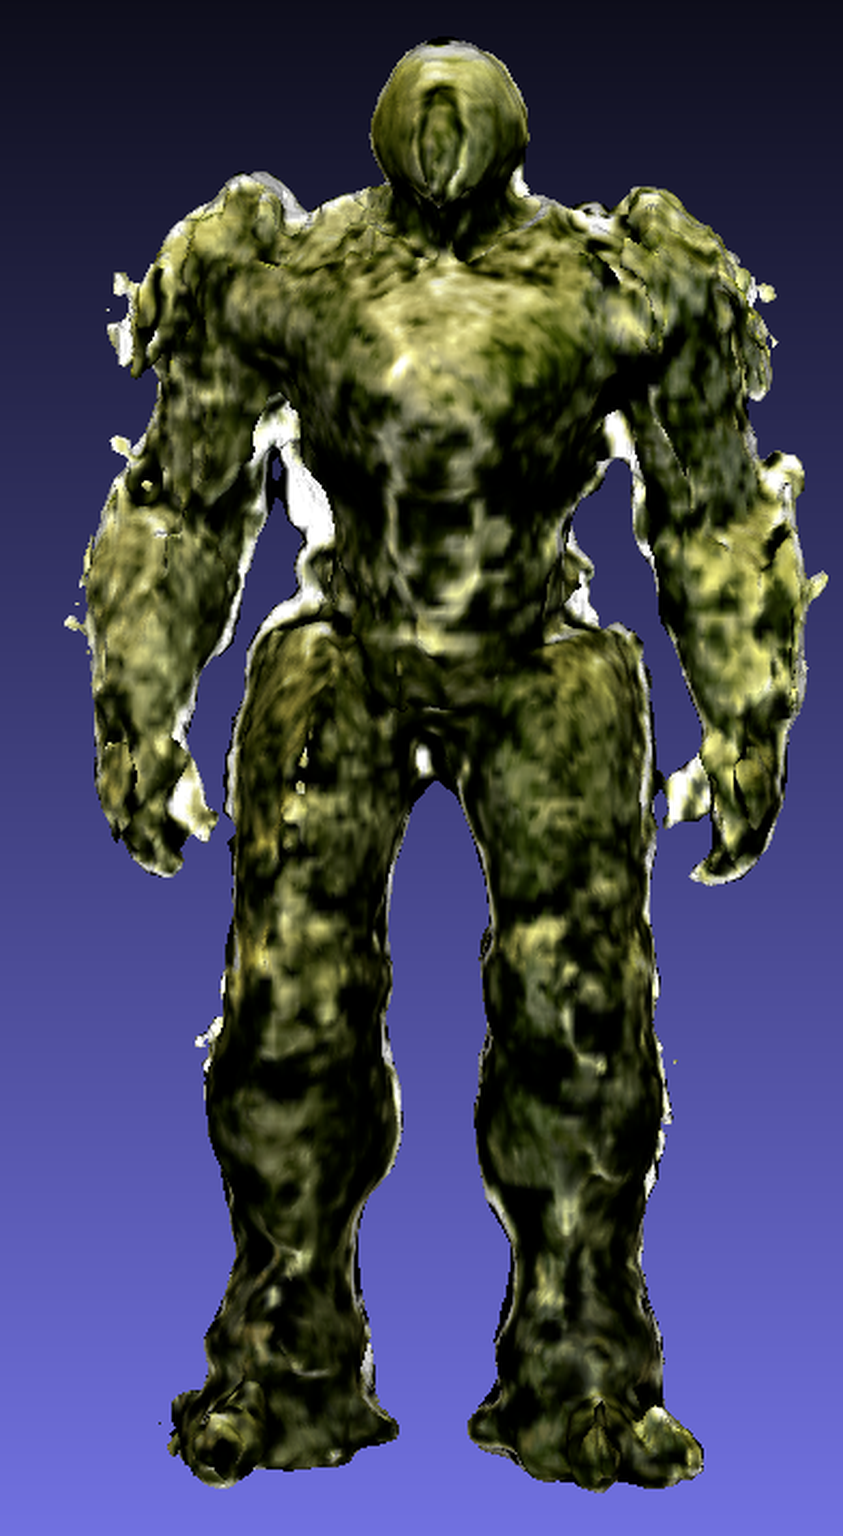
\includegraphics[width=\textwidth]{etc/a robot made out of plants/wonder3d/wonder3d_plantrobot_model_resized}
        \caption{Wonder3D}
    \end{subfigure}
    \caption{3D models generated by Magic123 and Wonder3D based on an imput image}~\label{fig:inputAndModel}
  \end{figure}
\textbf{Wonder3D}~--~This method operates by leveraging a Domain Switcher technique when provided with an image. It produces color images and normal maps from multiple viewpoints of the given image, ensuring consistency across these views. This approach is pivotal for obtaining a comprehensive understanding of the model, not just from the front perspective but from all angles. In this particular test, the same input image as used for Magic123 was employed, which can be viewed in Figure~\ref{fig:inputAndModel} part (b). Figure~\ref{fig:initializationWonder3D} in the appendix illustrates the six viewpoints generated by Wonder3D, including front, front-right, right, back, left, and front-left views, each accompanied by its respective normal maps and color images. Utilizing these outputs, the model strives to construct a coherent and consistent 3D representation.

Contrasting with other methods, Wonder3D does not currently provide detailed validation images throughout the training process. Instead, outputs are available only at intervals of every 3000 iterations, as depicted in Figure~\ref{fig:generationWonder3D}. From the available images, it is observed that the improvements in the model, based on the initially generated normals and color images, are relatively minor over the course of 10000 iterations. These slight enhancements are manifested in modest improvements in detail and the overall shape of the model, but they do not represent significant advancements from the initial stages.

\begin{figure}[H]
    \centering
    \begin{subfigure}[b]{0.18\textwidth}
        \centering
        \fontsize{9pt}{7pt}\selectfont\text{Iteration 0}
        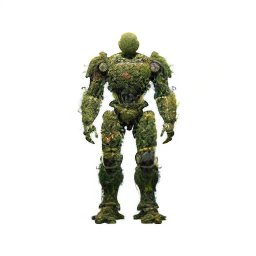
\includegraphics[width=\textwidth]{etc/a robot made out of plants/wonder3d/rgb_000_front}
        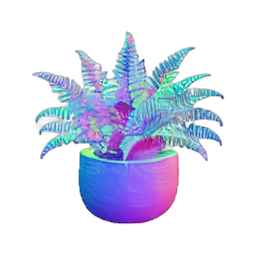
\includegraphics[width=\textwidth]{etc/a robot made out of plants/wonder3d/normals_000_front}
        \caption{}
    \end{subfigure}
    \begin{subfigure}[b]{0.18\textwidth}
        \centering
        \fontsize{9pt}{7pt}\selectfont\text{Iteration 3000}
        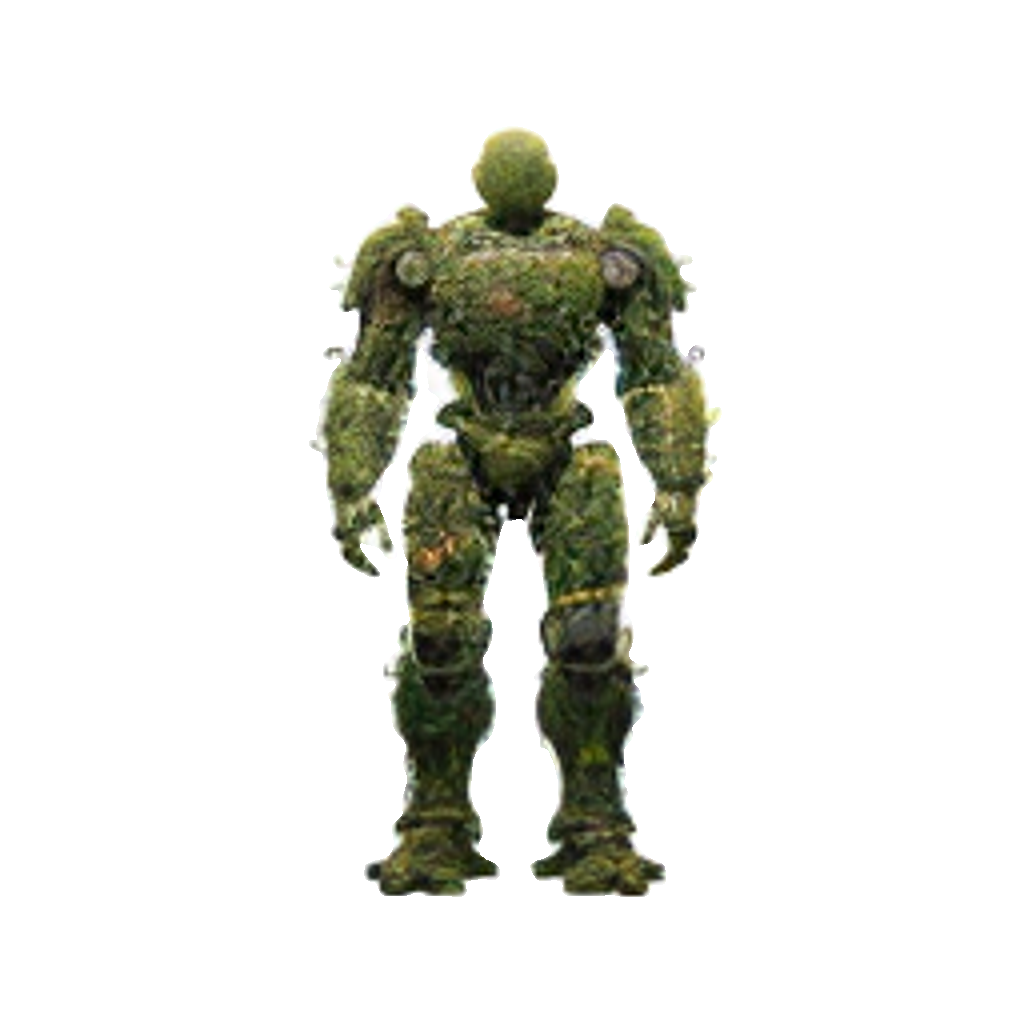
\includegraphics[width=\textwidth]{etc/a robot made out of plants/wonder3d/test/wonder3D_3000_front_part1}
        \includegraphics[width=\textwidth]{etc/a robot made out of plants/wonder3d/test/wonder3D_3000_front_part4}
        \caption{}
    \end{subfigure}
    \begin{subfigure}[b]{0.18\textwidth}
        \centering
        \fontsize{9pt}{7pt}\selectfont\text{Iteration 6000}
        \includegraphics[width=\textwidth]{etc/a robot made out of plants/wonder3d/test/wonder3D_6000_front_part1}
        \includegraphics[width=\textwidth]{etc/a robot made out of plants/wonder3d/test/wonder3D_6000_front_part4}
        \caption{}
    \end{subfigure}
    \begin{subfigure}[b]{0.18\textwidth}
        \centering
        \fontsize{9pt}{7pt}\selectfont\text{Iteration 9000}
        \includegraphics[width=\textwidth]{etc/a robot made out of plants/wonder3d/test/wonder3D_9000_front_part1}
        \includegraphics[width=\textwidth]{etc/a robot made out of plants/wonder3d/test/wonder3D_9000_front_part4}
        \caption{}
    \end{subfigure}
    \begin{subfigure}[b]{0.18\textwidth}
        \centering
        \fontsize{9pt}{7pt}\selectfont\text{Iteration 10000}
        \includegraphics[width=\textwidth]{etc/a robot made out of plants/wonder3d/test/wonder3D_10000_front_part1}
        \includegraphics[width=\textwidth]{etc/a robot made out of plants/wonder3d/test/wonder3D_10000_front_part4}
        \caption{}
    \end{subfigure}
    \caption{Wonder3D's results across different training iterations show that only minor changes occur throughout the process.}~\label{fig:generationWonder3D}
  \end{figure}
